\section{Background and Related Work}
\label{Background and Related Work}

    % \begin{table*}[h]
    % \label{related_work}
    % \caption{Conclusion table of related work}
    %     \center
    %     \begin{tabular}{|l|l|l|l|}
    %     \hline
    %     \multicolumn{1}{|c|}{\backslashbox{Methods~}{Goal~~}} & \multicolumn{1}{c|}{Access success prob} & \multicolumn{1}{c|}{Delay} & \multicolumn{1}{c|}{Energy consumption} \\
    %     \hline
    %     \multicolumn{1}{|c|}{ACB} & \multicolumn{1}{c|}{~\cite{cheng2011prioritized}~\cite{de2015random}~\cite{Ho2015Traffic}~\cite{giluka2013adaptive}~\cite{wang2014joint} } & \multicolumn{1}{c|}{~\cite{lien2012cooperative}  ~\cite{tribudi2015hybrid}} & \multicolumn{1}{c|}{} \\
    %     \hline
    %     \multicolumn{1}{|c|}{PRACH Separation} & \multicolumn{1}{c|}{} & \multicolumn{1}{c|}{~\cite{lee2011throughput}} & \multicolumn{1}{c|}{} \\
    %     \hline
    %     \multicolumn{1}{|c|}{DRA} & \multicolumn{1}{c|}{} & \multicolumn{1}{c|}{~\cite{shin2012radio}} & \multicolumn{1}{c|}{} \\
    %     \hline
    %     \multicolumn{1}{|c|}{SB} & \multicolumn{1}{c|}{~\cite{giluka2013adaptive} } & \multicolumn{1}{c|}{~\cite{jiang2014performance}} & \multicolumn{1}{c|}{} \\
    %     \hline
    %     \multicolumn{1}{|c|}{SA} & \multicolumn{1}{c|}{~\cite{cheng2011prioritized}~\cite{giluka2013adaptive}~\cite{sheu2012self}~\cite{madueno2014efficient} } & \multicolumn{1}{c|}{} & \multicolumn{1}{c|}{} \\
    %     \hline
    %     \multicolumn{1}{|c|}{PB} & \multicolumn{1}{c|}{} & \multicolumn{1}{c|}{~\cite{jiang2014performance}~\cite{wei2012dynamic}} & \multicolumn{1}{c|}{} \\
    %     \hline
    %     \multicolumn{1}{|c|}{Others} & \multicolumn{1}{c|}{~\cite{ko2012novel}} & \multicolumn{1}{c|}{} & \multicolumn{1}{c|}{~\cite{tu2011energy}} \\
    %     \hline
    %     \end{tabular}
    % \end{table*}

    \subsection{Random Access Procedure}
    \begin{figure}[t]
    \centering
    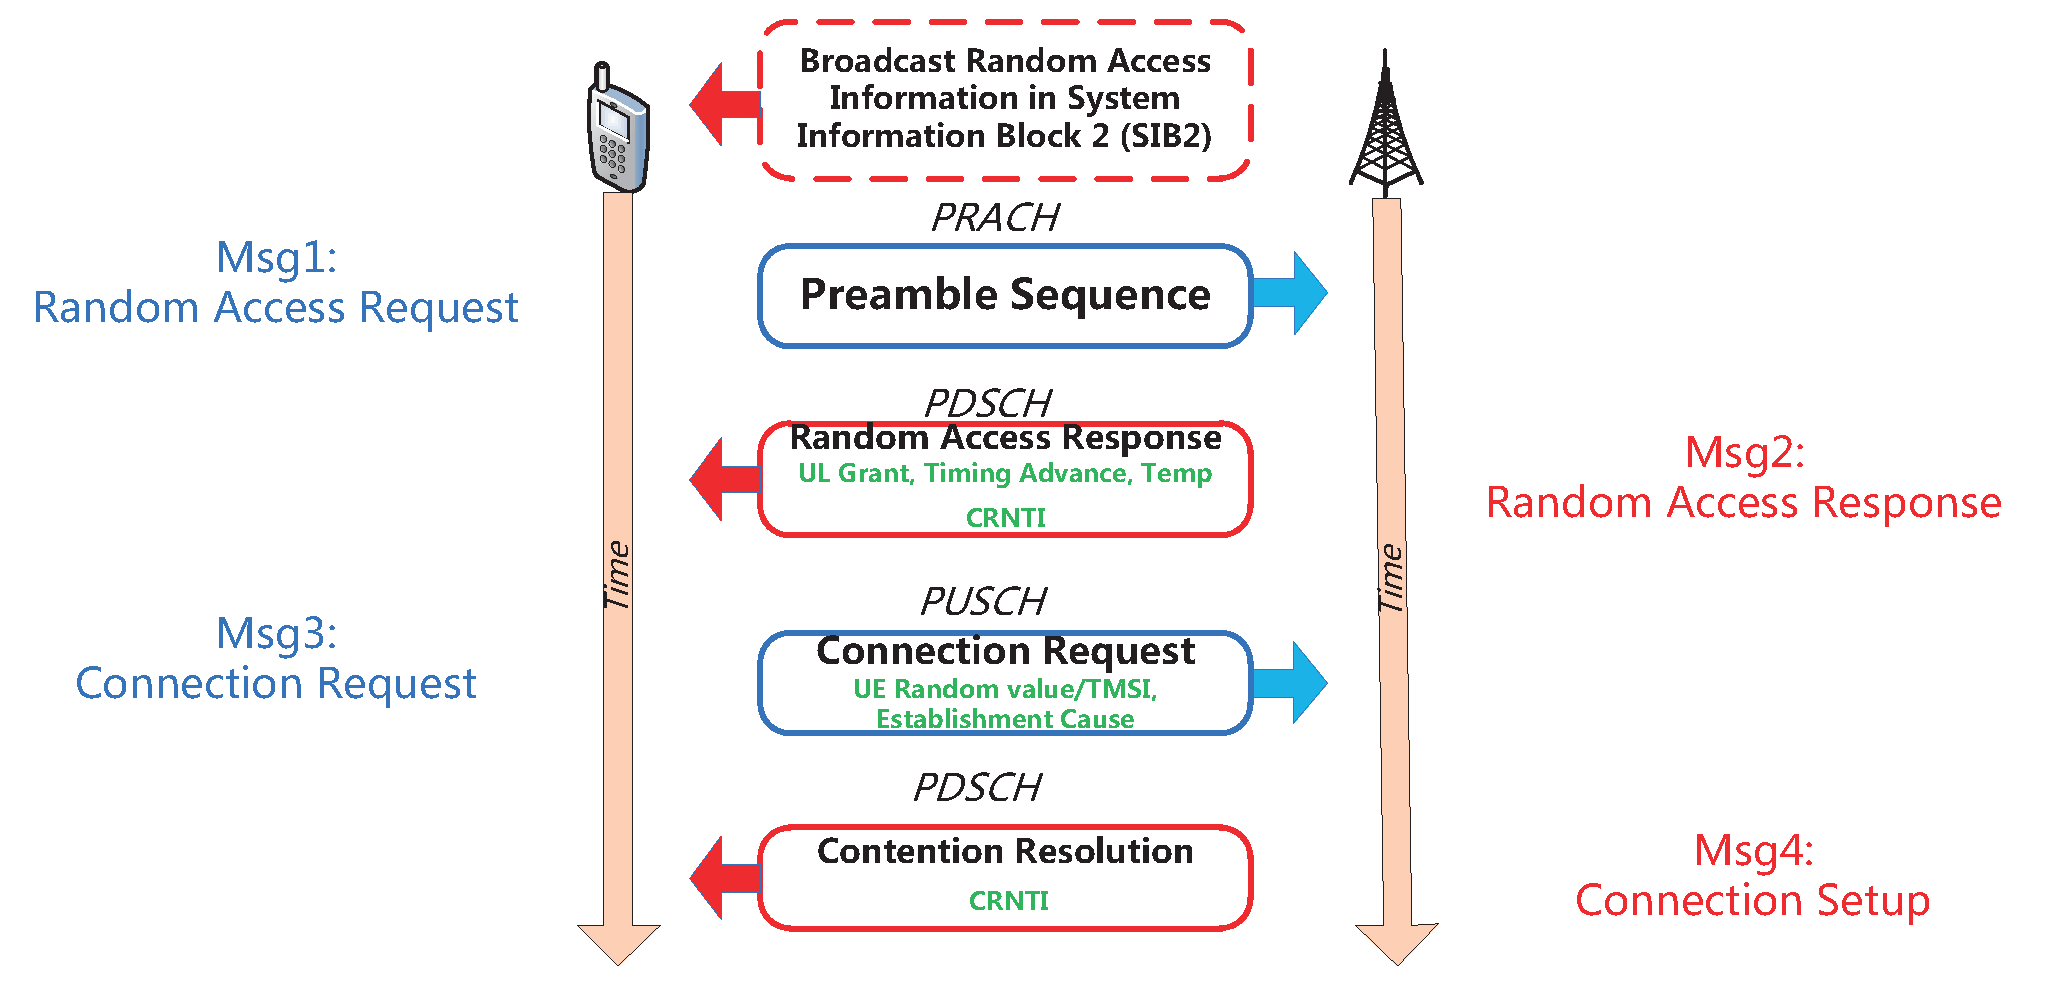
\includegraphics[width=3.8in]{fig_Rach_steps.eps}
    \caption{Random access 4 steps}
    \label{fig_RA_steps}
    \end{figure}

    While an UE device is switched on or handover from one eNB to another, it will perform random access procedure to contend resource blocks with others for data transmission. Random access procedure is classified into two types in LTE: contention based and contention free. In general, an UE device performs contention based random access procedure by randomly choosing a preamble. There are four steps in random access procedure shown in Fig.~\ref{fig_RA_steps}.

    \begin{itemize}
        \item
        Msg 1 called random access request, an UE device randomly chooses one of the available preambles and sends it to eNB on a physical random access channel (PRACH).
        \item 
        Msg 2 called random access response (RAR) contains an uplink scheduling grant for transmitting connection request, timing advance for synchronizing and temporary C-RNTI on the physical downlink shared channel (PDSCH).
        \item 
        In Msg 3, UE device will send its connection request to eNB on physical uplink shared channel (PUSCH) where is assigned by RAR. Therefore, those UEs who selected the same preamble will send their connection request on the same PUSCH and cause message collision because of receiving the same RAR from eNB.
        \item
        In Msg 4, the eNB will send contention resolution message to UE devices whose message was successfully received in Msg 3. This message contains the new C-RNTI which will be used for the further communication.
    \end{itemize}
    In this work, our focus lies in managing random access attempts to promote access success probability by using ACB scheme when congestion happening. The performance metrics of collision probability, access success probability are defined in~\cite{3GPP22.368}.


    \subsection{Related Work}
    \label{Related Work}
    When massive devices try to access the network simultaneously, it will cause RACH congestion because of the limited preamble in a PRACH slot and those devices who choose the same preamble will lead to collision in MSG 3. The congestion problem may rise intolerable delay and low access success probability so it has been considered as an essential issue in MTC. To reduce congestion in an overload condition, 3GPP~\cite{3GPP37.868} had proposed several basic solutions to solve the problem, which are described in the following subsection.
    \subsection{Basic Solving Congestion Solutions}
    \begin{itemize}
     \item Specific Backoff Scheme (SB)

            The scheme is suitable for normal load condition and the objective of the scheme is to reduce RACH congestion by delaying MTC devices. The backoff time for H2H will be set to a very small value, but the backoff time for MTC devices will be set to a very large value so as to let H2H have higher priority to access the network. 
            % In the work~\cite{jiang} a pre-backoff based random access (PBRA) scheme for group paging is proposed, some random access attempts of MTC devices are uniformly distributed by obtaining the pre-backoff information in paging message before the first preamble transmission.

     \item Slotted Access Scheme (SA)

            The access slots are defined for MTC devices and each MTC device can only access at its dedicated access slot. Furthermore, MTC devices will be in idle mode at other access slots.
            % The work in~\cite{sheu2012self} proposed a Self-Adaptive Persistent Contention mechanism (SPC) to schedule MTC devices in a periodical manner. The MTC devices only contend on MTC PRACH which is not used by H2H so that H2H devices will not be influenced by MTC devices.

     \item Pull Based Scheme (PB)

            A centralized manner, eNB sends the paging message to MTC devices whose data is required by MTC server. Upon receiving the paging message the MTC devices will initial random access procedure. Otherwise, MTC devices are not allowed to initial the procedure. 
            % Group paging~\cite{3GPP37.868} is another approach to solve the problem that we mentioned above. 
            % In~\cite{wei2012dynamic}, the work proposed a dynamic radio resource allocation algorithm for group paging approach in order to make the eNB assign a proper amount of radio resources to the networks.


      \item Dynamic PRACH Resource Allocation Scheme (DRA)

            In some scenarios the network can predict when access load will surge due to MTC devices. The eNB can dynamically allocate RACH resources for MTC devices to use according to RACH congestion level. 
            % In work~\cite{shin2012radio} proposed an adaptive radio resource control algorithm which can not only schedule the usage of radio resource but also reserve additional radio resource intended for messages that carry random backoff number for MTC devices.

      \item Access Class Barring Scheme (ACB)

            In ACB scheme, MTC devices are classified into several classes. eNB will broadcast access probability $p$ and backoff time corresponding to different access classes. Device will draw a value $q$, $0\leq q \leq 1$. If $q \leq p$, device is allowed to perform random access procedure. If the device is barred, it will start a backoff timer until end and a new attempt may be made. When congestion happens, the access probability $p$ can be set extremely small by eNB in order to bar the random access attempts, but the payoff of setting the extremely $p$ is that it may cause serious delay. The more detail of ACB can be studied in~\cite{3GPP22.011}.

            ~\cite{cheng2011prioritized} proposed QoS guaranteed prioritized random access scheme with a dynamic access barring scheme. Different virtual resource has been allocated for different classes in order to reduce the collision probability.

            ~\cite{de2015random} introduced the QoS-Aware Self-Adaptive RAN Overload Control (QoS-Dracon) mechanism to reduce the RAN overload problem, taking into account users’ QoS requirements. The QoS-Dracon scheme prioritizes delay-sensitive devices over delay-tolerant ones when performing Random Access procedure. It proposed a simple function based on the number of preamble transmissions of delay-sensitive devices to estimate the RAN load.

            ~\cite{Ho2015Traffic} developed a Markov-Chain based traffic-load estimation scheme according to the preamble collision status. With the estimation scheme, the eNB can adjust $p$ (ACB factor or Access probability) adaptively based on the overload situation. There are different simulation results compared with traditional ACB mechanism when setting different parameters used to update $p$. The results suggested the effectiveness of the traffic-aware ACB on the control of $p$ to balance the loads.

            ~\cite{jihun2016adaptive} and ~\cite{suyang2016dacb} proposed a mechanism to update ACB factor adaptively. The work in ~\cite{jihun2016adaptive} evaluate a congestion coefficient based on successful devices and contending device within each time region. And the ACB factor can be derived dynamically by the congestion coefficient. The work in ~\cite{suyang2016dacb} proposed an algorithm, which by using available information such as number of available preambles and number of successful preamble transmissions to dynamically update ACB factor.

            In summary, we made a conclusion of the mentioned papers and other related papers in table I. By observing the table and literature~\cite{de2015random}, ACB is the best way to solve RAN overload problem in above schemes because it is more flexible and efficient than the others. Due to the reason, we adopt ACB scheme and further modify the detail of this mechanism which will be described in section~\ref{proposed}.


    \end{itemize}
